
% \begin{figure}[t]
% 	\centering
%     % \vspace{-0.1cm} 
%     % \setlength{\abovecaptionskip}{0cm} 
%     % \setlength{\belowcaptionskip}{-0.2cm} 
% 	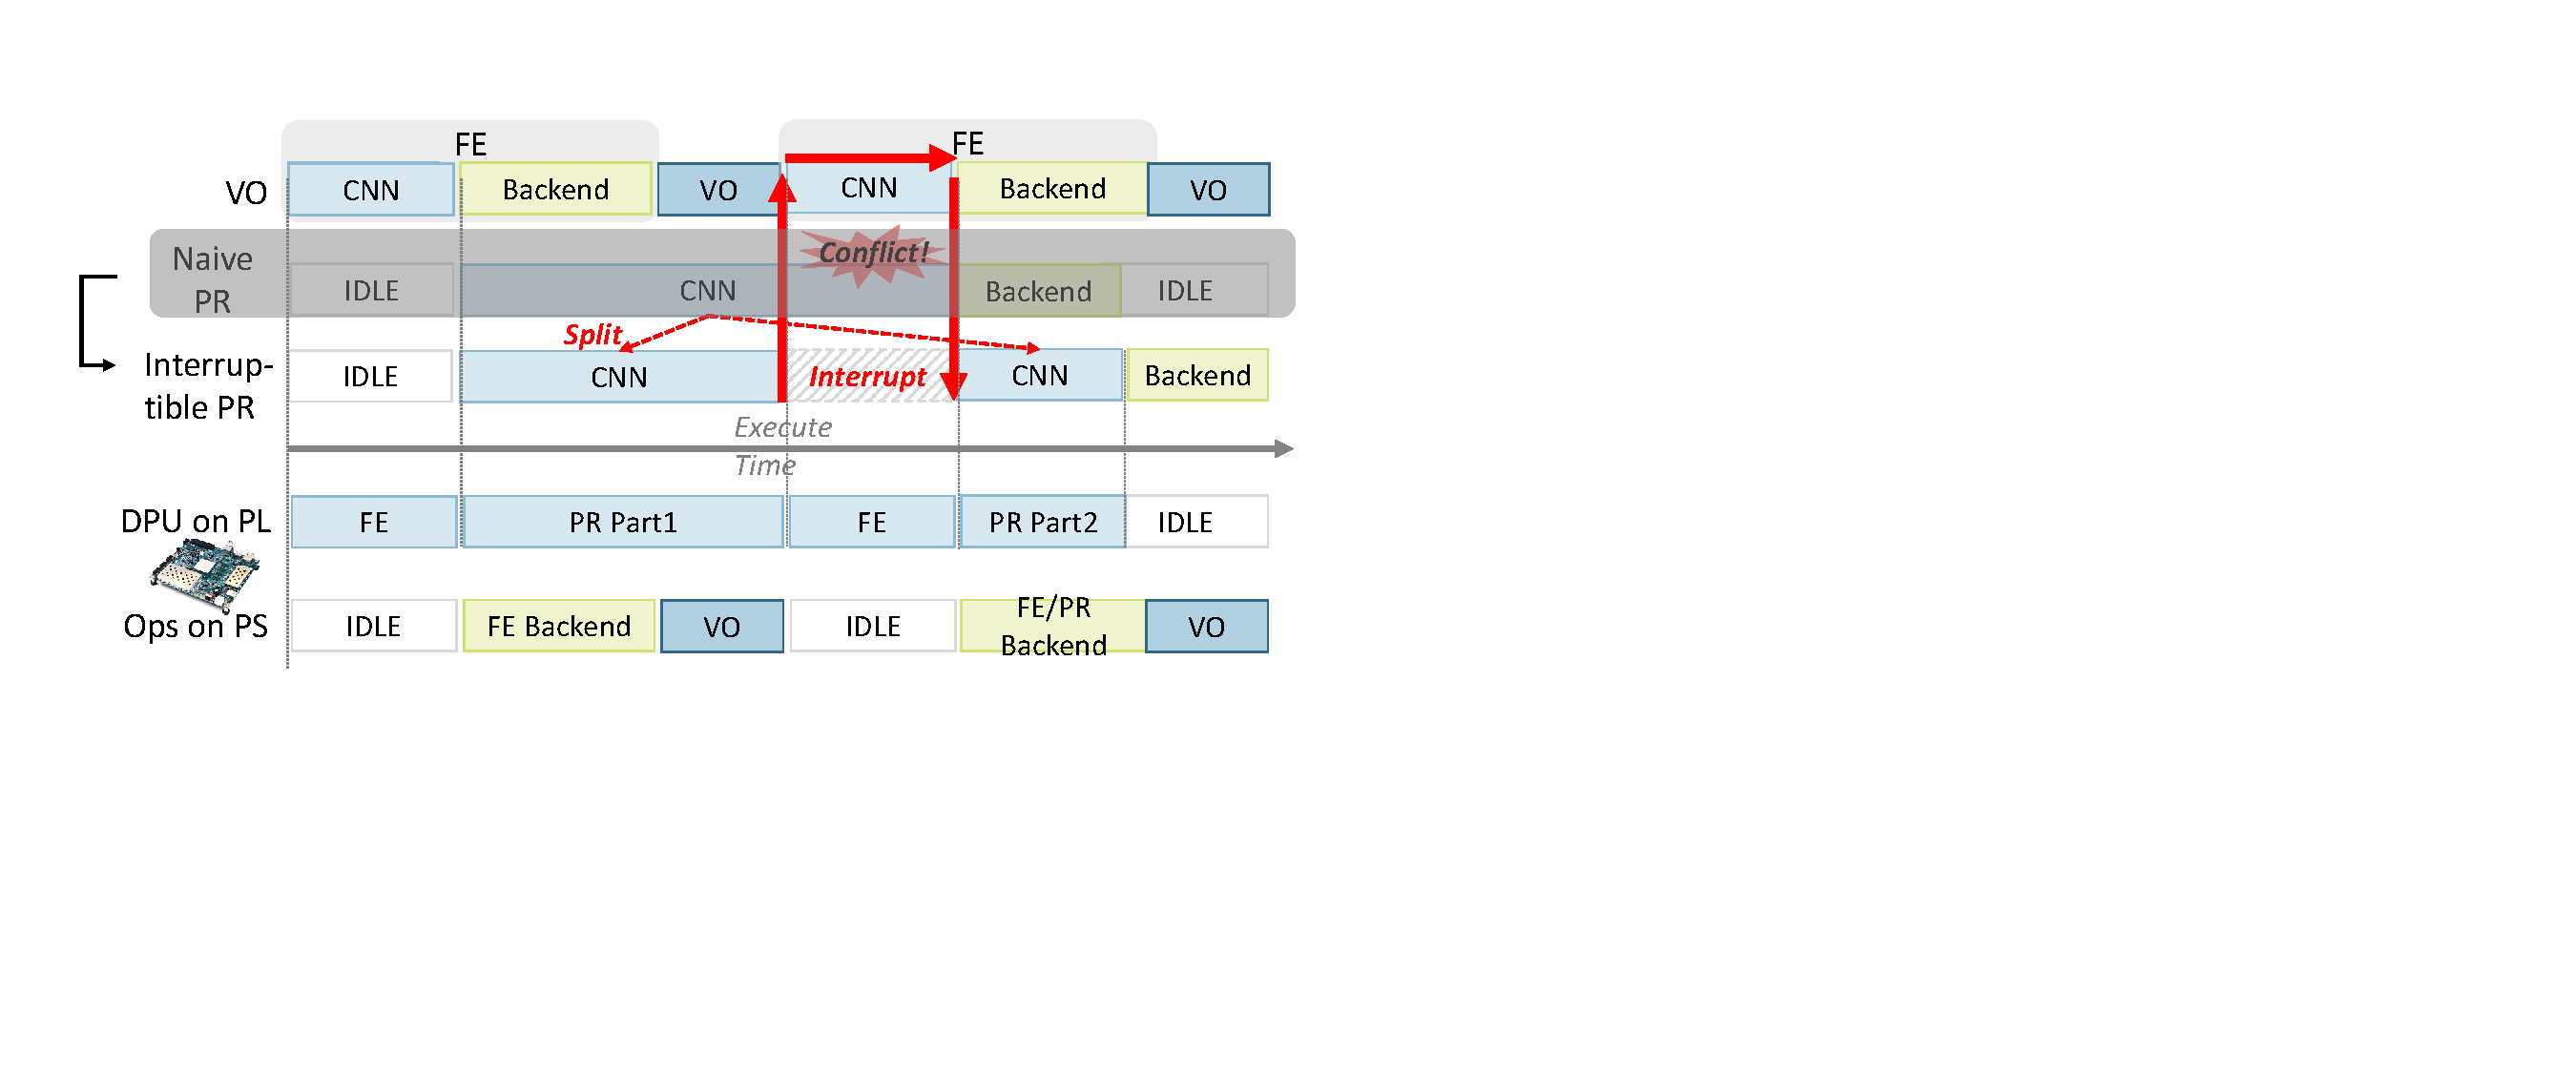
\includegraphics[width=0.95\linewidth]{fig/interDPR.pdf}
%     \caption{Interruption to solve the hardware resources conflicts.  
%     % When a high-priority task (FE) is started before the low-priority task (PR) is completed, the CNN accelerator backs up the status of PR to memory, and processes the FE task. When the high-priority task is completed, the low-priority task resumes and continues.
%     }
% 	\label{fig:interDPR}
% \end{figure}

% \begin{figure}[t]
% 	\centering
% 	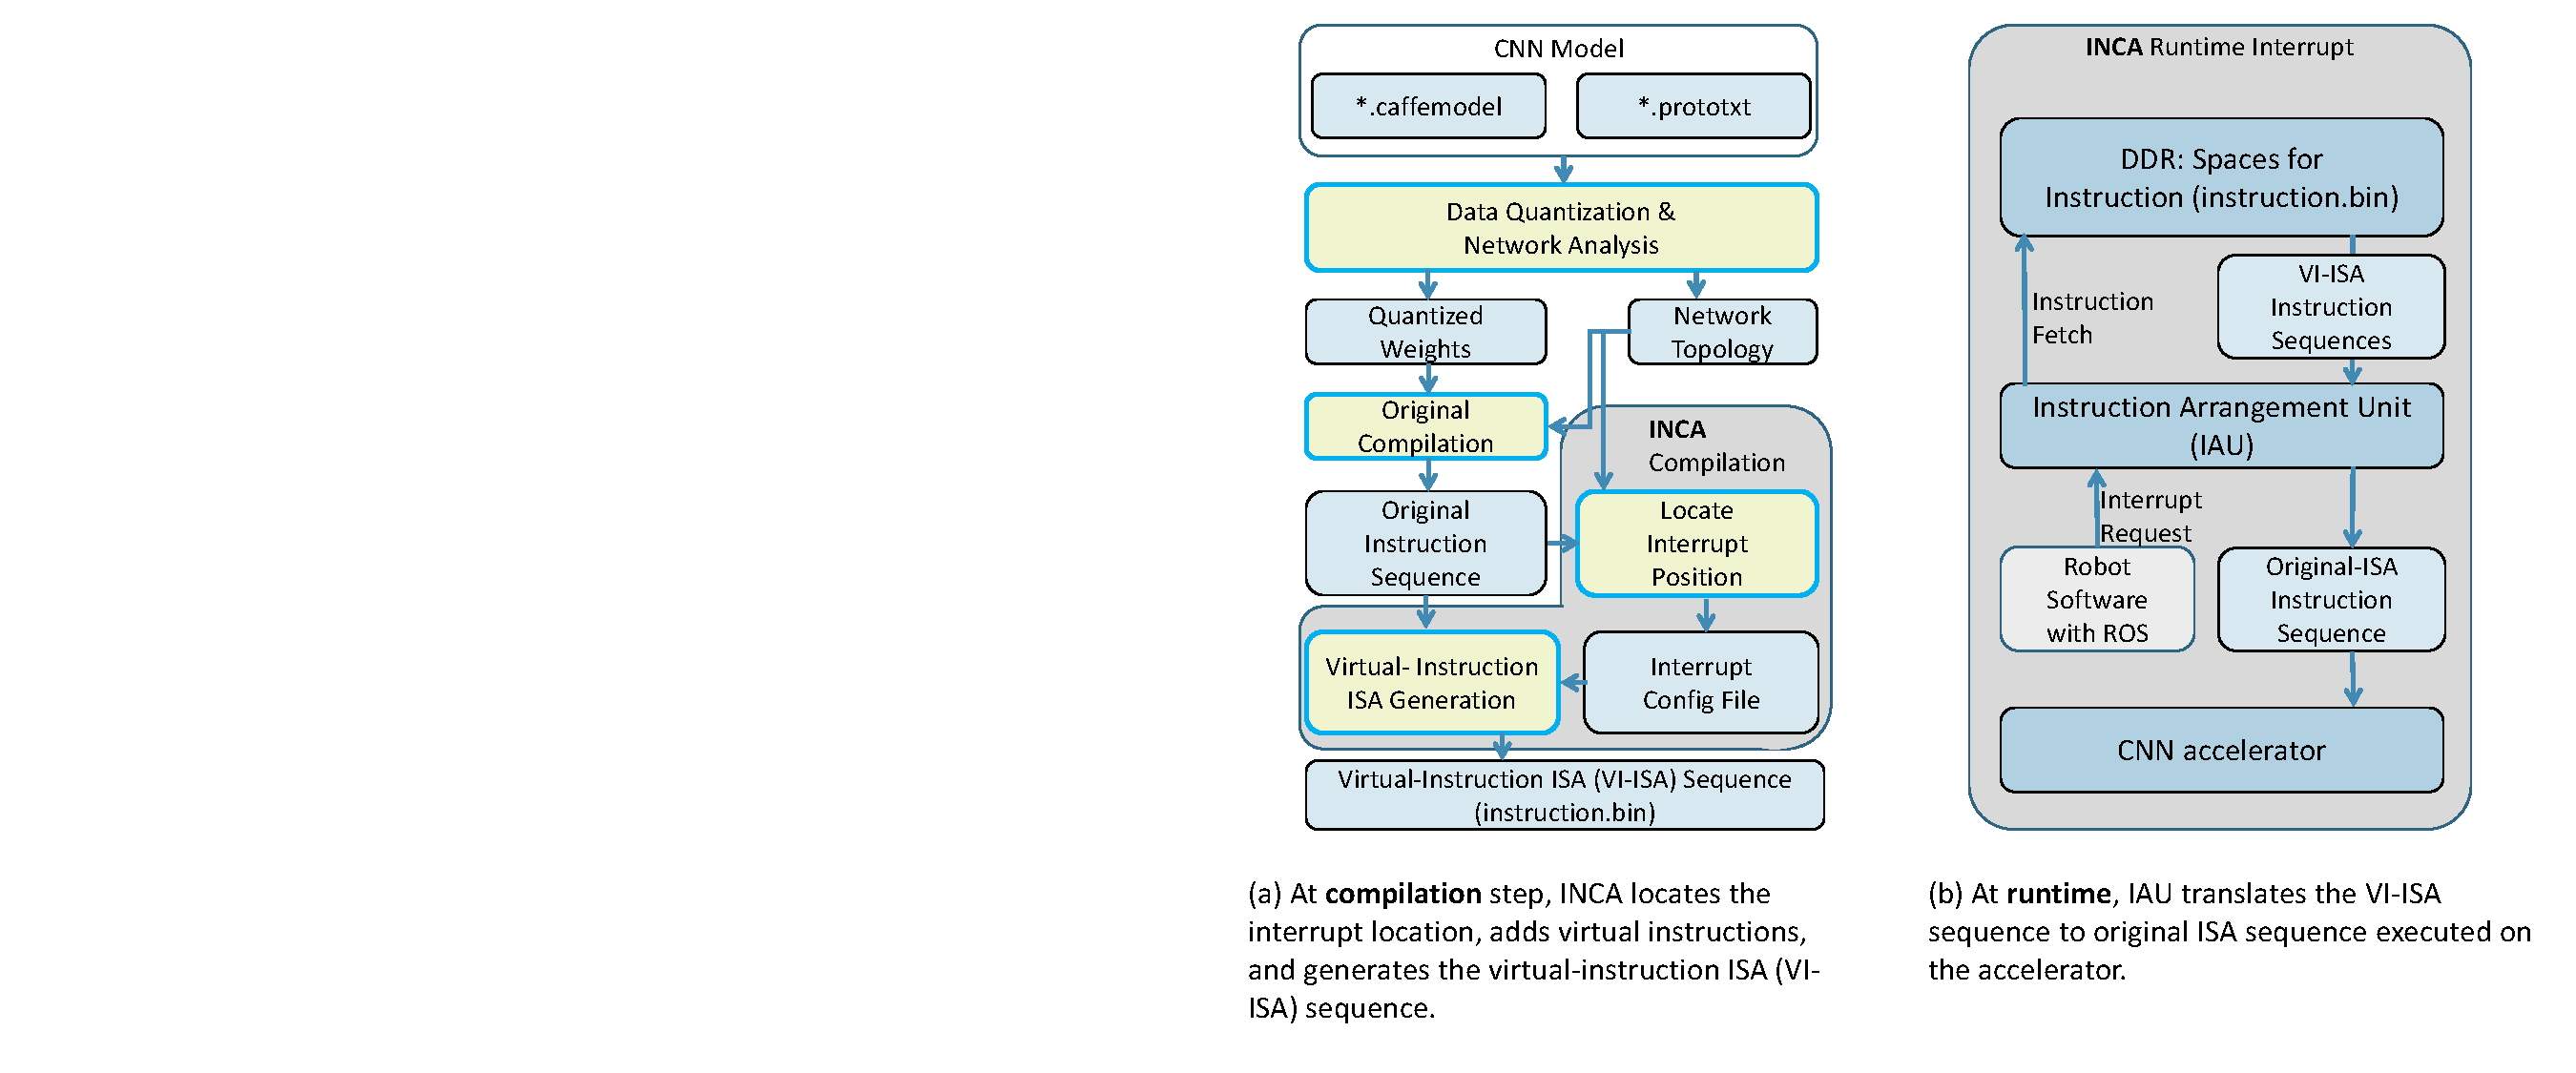
\includegraphics[width=0.95\linewidth]{fig/inca_acc.pdf}
%     \caption{INCA framework with Virtual-Instruction (VI).  
%     }
% 	\label{fig:inca_acc}
% \end{figure}


 Although ROS is becoming the fundamental software platform for robotics, the independence between different ROS nodes brings \textbf{hardware resources conflicts} to access the hardware accelerator. \Cref{fig:inca}(a) shows the time diagram of scheduling feature-point based visual odometry (VO) and Place Recognition in DSLAM system. The feature-point extraction (FE) and Place Recognition (PR) are impelmented in CNN and deployed to the CNN accelerator. In the native accelerator (the shadow part in  \Cref{fig:inca}(a)), the  threads  of  FE  and  PR  may  need  to  process  CNN  at  thesame  time,  and  the  simultaneous  requests  of  the  acceleratorwill  lead  to  hardware  resources  conflicts. 

\Cref{fig:inca}(a) also illustrates the idea of interrupt to schedule two CNN tasks. In the process of running a low-priority network (PR), the software may send an execution request for the high-priority task (FE). The interrupt enables the CNN accelerator to backup the running state of the low-priority PR network. Then the accelerator switches to the high-priority FE network. After the high-priority task (FE) completes, the low-priority task (PR) is restored to the accelerator and continues to execute.


\Cref{fig:inca}(c) details the INCA compilation step and runtime interrupt. Caffe  ~\cite{jia2014caffe} is a popular software framework for CNN, and the *.caffemodel/*.prototxt files define the network parameters and structure in Caffe. The previous deployment process, such as Angel-Eye  ~\cite{guo2017angel} and DPU ~\cite{dpu}, quantizes the weights, and analyze the network topology. The original compiler translates the network topology and the quantization information into the original ISA sequence. INCA goes further than previous CNN compilers. It selects the optimized interrupt positions in the original instruction sequence, and adds virtual instructions at these positions to enable accelerator interrupt. After that, the original instruction sequence and the added virtual instructions are wrapped to the new interruptible VI-ISA. The wrapped VI-ISA instructions are dumped into a file (instruction.bin), and can be loaded into the instruction spaces on FPGA's DDR.


As illustrated in \Cref{fig:inca}(d), at runtime, an Instruction Arrangement Unit (IAU) in hardware listens to the interrupt request from ROS software, fetches the corresponding VI-ISA interruptible instructions and translates them to the original ISA executed on the CNN accelerator. 
Although INCA can be applied to various instruction-based CNN accelerators, we implement and evaluate it based on Angel-Eye  ~\cite{guo2017angel}.
% The detail of the Virtual-Instruction ISA (VI-ISA) and instruction arrangement unit (IAU) is introduced in \Cref{sec:cnninterrupt}. Although INCA can be applied to various instruction-based CNN accelerators, we implement and evaluate it based on Angel-Eye  ~\cite{guo2017angel}.


